

%-------------------------------------------------------------------------------
% Dokumenten Klasse
\documentclass[
	final,
	a4paper,
	oneside,
	parskip=full,
	headings=standardclasses,
	headings=big,
	pointednumbers,
    fleqn
]{scrartcl}

%-------------------------------------------------------------------------------
% Packete nutzen
\usepackage{ngerman,palatino,setspace}
\usepackage[T1]{fontenc}
\usepackage[utf8]{inputenc}
\usepackage[left=20mm,right=20mm,top=10mm,bottom=25mm]{geometry}
\usepackage{amsmath}
\usepackage{amssymb}
\usepackage{mathtools}

%-------------------------------------------------------------------------------
\usepackage[dvipsnames]{xcolor}

%-------------------------------------------------------------------------------
% dbox
\usepackage{dashbox}

%-------------------------------------------------------------------------------
% uline
\usepackage{ulem}

%-------------------------------------------------------------------------------
% TikZ
\usepackage{tikz}
%\usetikzlibrary{positioning, arrows, decorations}
\usetikzlibrary{arrows,decorations.pathmorphing,backgrounds,positioning,fit,petri}

\tikzset{
    myptr/.style={
        ->,
        >=stealth
    }
}


%-------------------------------------------------------------------------------
% \ifthenelse
\usepackage{ifthen}

%-------------------------------------------------------------------------------
% Für enumerate
\usepackage{enumitem}
\setlist[enumerate]{
    wide=0pt,
    leftmargin=*,
    itemsep=-1ex,
    parsep=2ex,
    labelsep=1ex,
    label=\alph*)
}

\usepackage{multirow}
\usepackage{ifthen}

%-------------------------------------------------------------------------------
% tabu
\usepackage{tabu} 

%-------------------------------------------------------------------------------
% table line breaks with \makecell
\usepackage{makecell}
\renewcommand\cellalign{bl}

%-------------------------------------------------------------------------------
% 
\usepackage{xparse}
% 1: Subscription  (default: '')
% 2: Funktion Name (default: 'f')
% 3: Argument      (default: 'x')
% \fx         = f(x)
% \fx[1]      = f_1(x)
% \fx[][u]    = u(x)
% \fx[][u][x] = u(x)
% \fx[][f][u] = f(u)
\NewDocumentCommand{\fx}{ O{} O{f} O{x} }{{#2_{#1}{\left( #3 \right)}}}
\NewDocumentCommand{\dfx}{ O{} O{f} O{x} }{{#2'_{#1}{\left( #3 \right)}}}
\NewDocumentCommand{\dx}{ O{} }{{\Delta x^{#1}}}
\NewDocumentCommand{\dy}{ O{} }{{\Delta y^{#1}}}
\NewDocumentCommand{\dt}{ O{} }{{\Delta t^{#1}}}
\NewDocumentCommand{\gp}{ O{} }{}

\NewDocumentCommand{\xyz}{ O{x} O{y} O{z} }{#1 #2 #3}
% 1: Value
% 2: Key
% 3: Background Color
\NewDocumentCommand{\tfill}{ O{} O{} O{blue!20} }{%
    \tikz[baseline, every node/.style={inner sep=3pt,outer sep=0pt,minimum width=3mm,minimum height=4mm}]{
        \node[fill=#3,anchor=base] (#2) {#1};
    }
}
\NewDocumentCommand{\tfillc}{ O{} O{} }{%
    \tikz[baseline, every node/.style={inner sep=2pt,outer sep=0pt}]{
        \node[fill=#2,anchor=base] {#1};
    }
}

\NewDocumentCommand{\tdrawc}{ O{} O{} }{%
    \tikz[baseline, every node/.style={inner sep=2pt,outer sep=0pt}]{
        \node[rectangle,draw=#2,anchor=base] {#1};
    }
}
\newcommand{\tfillb}[1]{\tfillc[#1][blue!20]}
\newcommand{\tfillo}[1]{\tfillc[#1][orange!40]}
\newcommand{\tfillg}[1]{\tfillc[#1][Green!20]}
\newcommand{\tfilly}[1]{\tfillc[#1][yellow!40]}
\newcommand{\tfillr}[1]{\tfillc[#1][red!20]}
\newcommand{\tfillv}[1]{\tfillc[#1][Violet!20]}
\newcommand{\tfillt}[1]{\tfillc[#1][Turquoise!20]}
\newcommand{\tfillgr}[1]{\tfillc[#1][Gray!20]}


\newcommand{\tdrawb}[1]{\tdrawc[#1][blue!40]}
\newcommand{\tdrawo}[1]{\tdrawc[#1][orange!60]}
\newcommand{\tdrawg}[1]{\tdrawc[#1][Green!40]}
\newcommand{\tdrawy}[1]{\tdrawc[#1][yellow!60]}
\newcommand{\tdrawr}[1]{\tdrawc[#1][red!40]}
\newcommand{\tdrawv}[1]{\tdrawc[#1][Violet!40]}
\newcommand{\tdrawt}[1]{\tdrawc[#1][Turquoise!40]}
\newcommand{\tdrawgr}[1]{\tdrawc[#1][Gray!40]}
\newcommand{\tdrawk}[1]{\tdrawc[#1][black]}

% 1: Funktion Name
% 2: dx
% 3: dx^2
% 4: x_1
% 5: x_2
% 5: x_3
\NewDocumentCommand{\gpp}{ O{} O{\dx} O{\dx[2]} O{x} O{x} O{x} }{%
    \frac{1}{#3}
    \kl{#1 
        \kl{#4 \ifthenelse{\equal{#2}{}}{}{+ #2}} - 
        2 \cdot #1\kl{#5} +
        #1 \kl{#6\ifthenelse{\equal{#2}{}}{}{- #2}}
    }
}

% 1: x_1
% 2: x_2
% 3: x_3
% 4: dx^2
\NewDocumentCommand{\gppn}{ O{x_1} O{x_2} O{x_3} O{?}}{%
    \frac{1}{#4}
    \kl{#1 - 2 \cdot #2 + #3}
}

\newcommand*\difx{\; \mathop{}\!\mathrm{d}x}
\newcommand{\f}[2]{\frac{#1}{#2}}
%\newcommand{\fs}[2]{{\scriptstyle\frac{#1}{#2}}}
\newcommand{\fs}[2]{{\tfrac{#1}{#2}}}
\newcommand{\e}{\mathrm{e}}
\newcommand{\kl}[1]{{\left( #1 \right)}}
\newcommand{\kq}[1]{{\left\{ #1 \right\}}}
\newcommand{\ks}[1]{{\left[ #1 \right]}}
\newcommand{\dom}{{\Omega}}
\newcommand{\bound}{{\partial \Omega}}

%-------------------------------------------------------------------------------
% Dokument
\begin{document}

    \subsection*{Ableitungsregeln}
    
    \renewcommand{\arraystretch}{1.25}
    \begin{tabular}{lll}
        Faktorregel  & $ y = C \cdot \fx$                   & $ y' = C \cdot \dfx $ \\
                     & $ y = 5 \cdot x^2 $                  & $ y' = 5 \cdot 2 \cdot x$ \\
        Summenregel  & $ y = \fx[1] + \ldots +  \fx[n] $    & $ y' = \dfx[1] + \ldots + \dfx[n] $\\
                     & $ y = x^2 + x^3$                     & $ y' = 2 \cdot x + 3 \cdot x^2$ \\
        Produktregel & $ y = \fx[][u] \cdot \fx[][v] $      & $ y' = \fx[][u] \cdot \dfx[][v] + \dfx[][u] \cdot \fx[][v] $ \\
                     & $ y = x^2 \cdot e^{2x}  $            & $ y' = x^2 \cdot 2\cdot e^{2x} + 2\cdot x \cdot e^{2x} $ \\
                     &                                      & $ y' = {\left( 2x^2 + 2x \right)} e^{2x} $ \\
        Kettenregel  & $ y = f\kl{u\kl{x}} $                & $ y' = \dfx[][f][u] \cdot \dfx[][u][x] $ \\
                     & $ y = f\kl{x^2 - 5}, \; f = x^2 $    & $ y' = 2 u \cdot 2x = 4x \kl{x^2 - 5} $ \\
                     & $ y = \ln\kl{1 + x^2} $              & $ y' = \frac{1}{u} \cdot 2x = \frac{2x}{1 + x^2} $ \\
    \end{tabular} \\

    \renewcommand{\arraystretch}{1.25}
    \begin{tabular}{lll}
        Bestimmtes Integral & $ \int\limits_{a}^{b}{f\kl{x} \difx} $                      & $ = \ks{F\kl{x}}_{a}^{b} = F\kl{b} - F\kl{a} $ \\
        Faktorregel         & $ \int\limits_{a}^{b}{C \cdot f\kl{x} \difx} $              & $ = C \cdot \int\limits_{a}^{b}{f\kl{x} \difx} $     \\
        Summenregel         & $ \int\limits_{a}^{b}{\ks{f_1\kl{x} + f_2\kl{x}} \difx} $   & $ = \int\limits_{a}^{b}{f_1\kl{x} \difx} + \int\limits_{a}^{b}{f_2\kl{x} \difx} $      \\
        Zerlegungsregel     & $ \int\limits_{a}^{c}{f\kl{x} \difx} $                      & $ = \int\limits_{a}^{b}{f\kl{x} \difx} + \int\limits_{b}^{c}{f\kl{x} \difx}$  \\
    \end{tabular} \\

    %===================================================================================
    \newpage

    {\renewcommand{\arraystretch}{1.75}
    \begin{tabular}{ll}
        Forward FDM  & $g'\kl{x} = \frac{g \kl{x + \dx} - g \kl{x}}{\dx}$ \\
        Backward FDM & $g'\kl{x} = \frac{g \kl{x} - g \kl{x - \dx}}{\dx}$ \\
        Central FDM  & $g'\kl{x} = \frac{g \kl{x + \dx} - g \kl{x - \dx}}{2\dx}$
    \end{tabular}}

	\begin{minipage}{0.3\textwidth}
        \begin{align*}
            g'\kl{x}  &= \frac{g \kl{x + \dx} - g \kl{x}}{\dx} \\
            g''\kl{x} &= \frac{g \kl{x + \dx} - 2 \cdot g\kl{x} + g \kl{x - \dx}}{\dx[2]}
        \end{align*}
    \end{minipage}
	\begin{minipage}{0.7\textwidth}
        \begin{align*}
            u_{x}  &= \fs{1}{\dx}    \; \kl{u_{k+1} - u_{k}} \\
            u_{xx} &= \fs{1}{\dx[2]} \; \kl{u_{k+1} - 2\cdot u_{k} + u_{k-1}}
        \end{align*}
    \end{minipage}
    
    %===================================================================================
    \newpage
    
    %FDM with $\dx = \f{1}{\tikz[baseline]{\node[fill=blue!20,anchor=base] (t1) {$5$};}} = \f{1}{\tikz[baseline]{\node[fill=blue!20,anchor=base] (t1) {$n$};}} $
    
    \tikzstyle{every picture}+=[remember picture]
    FDM with $\dx = \f{1}{\tfill[$\scriptstyle{5}$][frac1][blue!20]} = \f{1}{\tfill[$\scriptstyle{n}$][frac2][red!20]} $
    %\tfill[5][p5][red]
    %\xyz[a][b][c]

    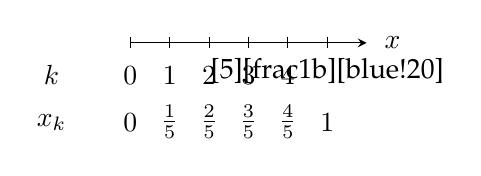
\begin{tikzpicture}[
        ]
        % draw horizontal line   
        \draw[myptr] (0,0) -- (3,0) node[right=3pt] {$x$};
        
        % draw vertical lines
        \foreach \k in {0, 1, 2, 3, 4, 5}
        {
            \ifthenelse{\NOT 0 = \k \AND \NOT 5 = \k}{
                \draw (\k*0.5 cm,2pt) -- (\k*0.5 cm,-2pt)  node[below=3pt] (k\k) {$\k$} node[below=20pt,shift={(0,3pt)}] (xk\k) {$\frac{\k}{5}$};
            }{
                \ifthenelse{5 = \k}{
                    \draw (\k*0.5 cm,2pt) -- (\k*0.5 cm,-2pt)  node[below=3pt,shift={(0,3pt)}] (k\k) {\tfill[5][frac1b][blue!20]} node[below=20pt] (xk\k) {$1$};
                }{
                    \draw (\k*0.5 cm,2pt) -- (\k*0.5 cm,-2pt)  node[below=3pt] (k\k) {$\k$} node[below=20pt] (xk\k) {$\k$};
                }
            }
        }
        \node[left of=k0] {$k$};
        \node[left of=xk0] {$x_k$};
        % draw nodes
    \end{tikzpicture}
    \begin{tikzpicture}[overlay]
        \draw[color=blue!60] (frac1b) -- (frac1);
    \end{tikzpicture}
    
    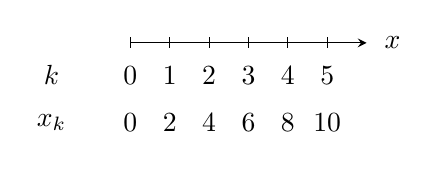
\begin{tikzpicture}[
        ]
        % draw horizontal line   
        \draw[myptr] (0,0) -- (3,0) node[right=3pt] {$x$};
        
        % draw vertical lines
        \foreach \k/\xk in {0/0, 1/2, 2/4, 3/6, 4/8, 5/10}
        {
            \draw (\k*0.5 cm,2pt) -- (\k*0.5 cm,-2pt)  node[below=3pt] (k\k) {$\k$} node[below=20pt] (xk\k) {$\xk$};
        }
        \node[left of=k0] {$k$};
        \node[left of=xk0] {$x_k$};
        % draw nodes
    \end{tikzpicture}

    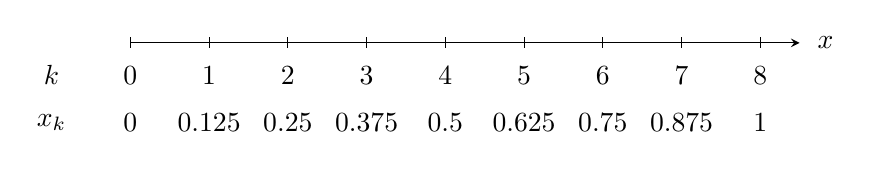
\begin{tikzpicture}[
        ]
        % draw horizontal line   
        \draw[myptr] (0,0) -- (8.5,0) node[right=3pt] {$x$};
        
        % draw vertical lines
        \foreach \k/\xk in {0/0, 1/0.125, 2/0.25, 3/0.375, 4/0.5, 5/0.625, 6/0.75, 7/0.875, 8/1}
        {
            \draw (\k cm,2pt) -- (\k cm,-2pt)  node[below=3pt] (k\k) {$\k$} node[below=20pt] (xk\k) {$\xk$};
        }
        \node[left of=k0] {$k$};
        \node[left of=xk0] {$x_k$};
        % draw nodes
    \end{tikzpicture}



    sss

	\begin{minipage}[t]{0.09\textwidth}
        $x_1$
	\end{minipage}
	\begin{minipage}[t]{0.91\textwidth}
        \begin{align*}
            \gpp[\widetilde{T}][2][2^2][x_1][x_1][x_1] & \\
            \gpp[\widetilde{T}][][2^2][x_2][x_1][x_0] & \\
            \gppn[T_2][T_1][T_0][2^2] & \\
            \gppn[40][T_1][T_0][2^2] &
        \end{align*}
	\end{minipage}

    
    \begin{tabular}{lll}
        \text{{\color{blue}\uline{Hyperpolic}}} & & \text{{\color{red}\uline{Parabolic}}} \\
        $ {\color{blue}r = \f{\dt}{\dx}} $      & ${\color{red}\neq}$ & ${\color{red}r = \f{\dt}{\dx[2]}}$
    \end{tabular}

    

    

    $ \Delta u=u_{xx}+u_{yy}=0 $

    $\Delta u=u_{xx}+u_{yy}=f(x,y)$

    $ \Delta u =  u_{xx} + u_{yy} = \frac{\partial^2 u}{\partial x^2} + \frac{\partial^2 u}{\partial y^2} = 0 $

    \begin{tabular}{ll}
        Nabla Operator                  & $\nabla{u} = u_{x}+u_{y} = \frac{\partial u}{\partial x} + \frac{\partial u}{\partial y}$ \\
        Laplace Operator                & $\Delta{u} = u_{xx} + u_{yy} = \frac{\partial^2 u}{\partial x^2} + \frac{\partial^2 u}{\partial y^2} $\\
        \hline
        \hline
        Anfangswertproblem (AWP)        & \multirow{2}{*}{$u\kl{x,0} = f\kl{x}, \quad {\textstyle\f{\partial u}{\partial x}}\kl{x,0} = g\kl{x}$} \\
        Initial value problem (IVP)     & \\
        \hline
        Randwertproblem (RWP)           & \multirow{2}{*}{$u\kl{x,a} = \alpha, \quad u\kl{x,b} = \beta $} \\
        Boundary value problem (BVP)    & \\
        \hline
        Dirichlet-Randbedingung         & $u\kl{x,0} = f\kl{x}$ \\
        Dirichlet boundary condition    & Werte auf dem Rand liegend \\
        \hline
        Neumann-Randbedingung           & ${\textstyle\f{\partial u}{\partial x}}\kl{x,0} = f\kl{x}$ \\
        Neumann boundary condition      & Ableitungswerte auf dem Rand liegend \\
        \hline
        Laplace-Gleichung               & \multirow{2}{*}{$\Delta u = 0 $}\\
        Laplace's equation              & \\
        \hline
        Poisson-Gleichung               & \multirow{2}{*}{$-\Delta u = f $}\\
        Poisson's equation              &
    \end{tabular}

    \begin{tabular}{lll}
        \multicolumn{3}{c}{$ Au_{xx} + 2Bu_{xy} + Cu_{yy} + Du_x + Eu_y + Fu +G= 0 $} \\
        \hline
        Elliptische PDF                 & Laplace-/Poisson-Gleichung    & \multirow{2}{*}{$ B^2 - AC < 0$} \\
        Elliptic PDE                    & Laplace-/Poisson's equation   & \\
        \hline
        Parabolische PDF                & Wärmeleitungsgleichung, Diffusionsgleichung   & \multirow{2}{*}{$ B^2 - AC = 0$} \\
        Parabolic PDE                   & Heat Equation, Diffusion Equation             & \\
        \hline
        Hyperbolische PDF               & Transportgleichung, Wellengleichung           & \multirow{2}{*}{$ B^2 - AC < 0 $} \\
        Hyperbolic PDE                  & Advection Equation, Wave Equation             &
    \end{tabular}

    \begin{tabular}{ll}
        \hline
        Elliptische PDF                 & Laplace-/Poisson-Gleichung                    \\
        Elliptic PDE                    & Laplace-/Poisson's equation                   \\
        \hline
        Parabolische PDF                & Wärmeleitungsgleichung, Diffusionsgleichung   \\
        Parabolic PDE                   & Heat Equation, Diffusion Equation             \\
        \hline
        Hyperbolische PDF               & Transportgleichung, Wellengleichung           \\
        Hyperbolic PDE                  & Advection Equation, Wave Equation             
    \end{tabular}


    %===================================================================================
    \newpage

    \subsection*{Finite Difference Method (FDM)}
    \subsection*{Elliptic PDEs}

    \subsubsection*{Dirichlet Boundary Conditions}
    
    Discrete Laplace-Operator / 5-Star-Operator
    
    \begin{align*}
        \Delta u & = u_{xx} + u_{yy} \\
        h        & = \dx = \dy \\
        \Delta u & \approx \f{1}{h^2} \kq{u\kl{x + h, y} + u\kl{x, y + h} + u\kl{x - h, y} + u\kl{x, y - h} - 4 \cdot u\kl{x,y}} \\
        \Delta u & \approx \f{1}{h^2} \kq{u\kl{P_E} + u\kl{P_N} + u\kl{P_W} + u\kl{P_S} - 4 \cdot u\kl{P_C}}
    \end{align*}

    \subsubsection*{Neumann Boundary Conditions}

    \begin{align*}
        u_x\kl{P_C} & \approx \f{u\kl{P_E} - u\kl{P_W}}{2\cdot h} \\
        u\kl{P_W}   & = u\kl{P_E} - 2\cdot h \cdot u_x\kl{P_C} \\
        \Delta u    & \approx \f{1}{h^2} \kq{u\kl{P_E} + u\kl{P_N} + \tfillr{$u\kl{P_W}$} + u\kl{P_S} - 4 \cdot u\kl{P_C}} \\
                    & \approx \f{1}{h^2} \kq{u\kl{P_E} + u\kl{P_N} + \tfillr{$u\kl{P_E} - 2\cdot h \cdot u_x\kl{P_C}$} + u\kl{P_S} - 4 \cdot u\kl{P_C}} \\
                    & \approx \f{1}{h^2} \kq{\tfillr{$2$} \cdot u\kl{P_E} + u\kl{P_N} + u\kl{P_S} - 4 \cdot u\kl{P_C} \tfillr{$- 2\cdot h \cdot u_x\kl{P_C}$}} \\
    \end{align*}
    

    
    %===================================================================================
    \newpage

    \subsection*{Parabolic PDEs}
    \subsubsection*{Richardson's Explicit Method}

    \begin{align*}
        u_{t}\kl{x,t}                               & = u_{xx}\kl{x,t} \\
        u_{\dt + 1} & = \ks{\ldots}  u_{\dt}
    \end{align*}
    
    Forward Finite Difference in $t$ and $x$ \\
    {\setlength{\abovedisplayskip}{-6pt}
    \setlength{\belowdisplayskip}{-12pt}
    \begin{align*}
        % 1
        \f{u \kl{x, t + \dt} - \tfillb{$u \kl{x, t}$}}{\dt}    & = \f{
            \tfillr{$u \kl{x + \dx, t}$} -
            2 \cdot \tfillg{$u\kl{x, t}$} +
            \tfilly{$u \kl{x - \dx, t}$}
        }{\dx[2]}, \quad \tfillo{$r$}   = \f{\dt}{\dx[2]}  \\
        % 2
        u \kl{x, t + \dt} & = \tfillo{$r$} \cdot \kq{
            \tfillr{$u \kl{x + \dx, t}$} -
            2 \cdot \tfillg{$u\kl{x, t}$} +
            \tfilly{$u \kl{x - \dx, t}$}
        } + \tfillb{$u \kl{x, t}$} \\
        % 3
        u_{x,t+1} & = \tfillo{$r$} \cdot \kq{u_{x+1,t} - 2 \cdot u_{x,t} + u_{x-1,t}} + \tfillb{$u \kl{x, t}$} \\
        u_{x,t+1} & = \tfillo{$r$} \cdot \tfilly{$u_{x-1,t}$} + \kl{\tfillb{$1$} - \tfillg{$2\cdot r$}} \cdot u_{x,t} + \tfillo{$r$} \cdot \tfillr{$u_{x+1,t}$} \\
        u_{j,k+1} & = \tfillo{$r$} \cdot \tfilly{$u_{j-1,k}$} + \kl{\tfillb{$1$} - \tfillg{$2\cdot r$}} \cdot u_{j,k} + \tfillo{$r$} \cdot \tfillr{$u_{j+1,k}$} \\
        \uline{u}^{k+1} &= C \cdot \uline{u}^{k} \\
        \uline{u}^{k} &= \kq{C}^{k} \cdot \uline{u}^{0}
    \end{align*}}


    \subsubsection*{Richardson's Implicit Method}
    
    Backward Finite Difference in $t$, Forward Finite Difference $x$ \\
    {\setlength{\abovedisplayskip}{-6pt}
    \setlength{\belowdisplayskip}{-12pt}
    \begin{align*}
        % 1
        \f{\tfillb{$u \kl{x, t}$} - u \kl{x, t - \dt} }{\dt} & = \f{
            \tfillr{$u \kl{x + \dx, t}$} -
            2 \cdot \tfillg{$u\kl{x, t}$} +
            \tfilly{$u \kl{x - \dx, t}$}
        }{\dx[2]}, \quad \tfillo{$r$}   = \f{\dt}{\dx[2]}  \\
        % 2
        u \kl{x, t - \dt} & = \tfillb{$u \kl{x, t}$} - \tfillo{$r$} \cdot \kq{
            \tfillr{$u \kl{x + \dx, t}$} -
            2 \cdot \tfillg{$u\kl{x, t}$} +
            \tfilly{$u \kl{x - \dx, t}$}
        } \\
        % 3
        u_{x,t-1} & = \tfillb{$u \kl{x, t}$} -\tfillo{$r$} \cdot \kq{u_{x+1,t} - 2 \cdot u_{x,t} + u_{x-1,t}} \\
        u_{x,t-1} & = -\tfillo{$r$} \cdot \tfilly{$u_{x-1,t}$} + \kl{\tfillb{$1$} + \tfillg{$2\cdot r$}} \cdot u_{x,t} - \tfillo{$r$} \cdot \tfillr{$u_{x+1,t}$} \\
        u_{j,k-1} & = -\tfillo{$r$} \cdot \tfilly{$u_{j+1,k}$} + \kl{\tfillb{$1$} + \tfillg{$2\cdot r$}} \cdot u_{j,k} - \tfillo{$r$} \cdot \tfillr{$u_{j+1,k}$} \\
        \uline{u}^{k} &= E \cdot \uline{u}^{k+1} \\
        \uline{u}^{k+1} &= E^{-1}\cdot \uline{u}^{k} \\
        \uline{u}^{k} &= \kq{E^{-1}}^{k} \cdot \uline{u}^{0}
    \end{align*}}

    \subsubsection*{Method of Crank-Nicolson}
    $\fs{1}{2}$ Explicit, $\fs{1}{2}$ Implicit + $\dt$ \\
    {\setlength{\abovedisplayskip}{-6pt}
    \setlength{\belowdisplayskip}{-12pt}
    \begin{align*}
        % Explicit
        \f{\tfillt{$u \kl{x, t + \dt}$} - \tfillb{$u \kl{x, t}$} }{\dt}    & = \f{
            u \kl{x + \dx, t} -
            2 \cdot u\kl{x, t} +
            u \kl{x - \dx, t}
        }{\dx[2]} \\
        % Implicit + dt
        \f{\tfillt{$u \kl{x, t + \dt}$} - \tfillb{$u \kl{x, t}$} }{\dt} & = \f{
            u \kl{x + \dx, t + \dt} -
            2 \cdot u\kl{x, t + \dt} +
            u \kl{x - \dx, t + \dt}
        }{\dx[2]} \\
        % Method of Crank-Nicolson
        % left
        -\tfillo{$r$} \cdot u_{j-1,\tfilly{$\scriptstyle k+1$}}                 \tfillgr{$+$}
        \kl{2 + 2\cdot \tfillo{$r$} } \cdot u_{j,\tfilly{$\scriptstyle k+1$}}   \tfillgr{$-$}
        \tfillo{$r$}  u_{j+1,\tfilly{$\scriptstyle k+1$}}                       & =
        % right
        \tfillo{$r$} \cdot u_{j-1,\tfillg{$\scriptstyle k$}}                    \tfillgr{$+$}
        \kl{2 - 2\cdot \tfillo{$r$}} \cdot u_{j,\tfillg{$\scriptstyle k$}}      \tfillgr{$+$}
        \tfillo{$r$} \cdot u_{j+1,\tfillg{$\scriptstyle k$}}
    \end{align*}}

    %===================================================================================
    \newpage

    \subsection*{Hyperbolic PDEs}
    \subsubsection*{Advection Equation / Transportgleichung}
    
    {\it{Problem 70}} \\
    \begin{tabular}{p{5cm}l}
        Domain $\dom$                 & $\Omega = \kl{-\infty, \infty} \times \left[ 0, \infty \right)$ \\
        Advection Equation              & $u_x\kl{x,t} + u_t\kl{x,t} = 0$ \\
        Dirichlet boundary-condition on $\bound$    & $u\kl{x,0} = f\kl{x}$
    \end{tabular}

    {\bf{Downwind Scheme}} \\
    Forward Finite Difference in $t$ and $x$ \\
    {\setlength{\abovedisplayskip}{-6pt}
    \setlength{\belowdisplayskip}{-12pt}
    \begin{align*}
        \f{u \kl{x,\;t + \dt} - u \kl{x, t}}{\dt} &+ \f{ \tfilly{$u \kl{x + \dx, t}$} - u\kl{x, t}}{\dx} = 0 \\
        u_{j,k+1} - \tfillb{$u_{j,k}$}  &= \tfillo{${\fs{\dt}{\dx}}$} \kq{u_{j,k} - \tfilly{$u_{j+1,k}$}} \\
        u_{j,k+1}                       &= \tfillo{$r$} \cdot \kq{u_{j,k} - \tfilly{$u_{j+1,k}$}} + \tfillb{$u_{j,k}$} \\
        u_{j,k+1}                       &= \kl{\tfillb{$1$}+\tfillo{$r$}} \cdot u_{j,k} - \tfillo{$r$} \cdot \tfilly{$u_{j+1,k}$}
    \end{align*}}

    {\bf{Upwind Scheme}} \\
    Forward Finite Difference in $t$, Backward Finite Difference in $x$ \\
    {\setlength{\abovedisplayskip}{-6pt}
    \setlength{\belowdisplayskip}{-12pt}
    \begin{align*}
        \f{u \kl{x,\;t + \dt} - u \kl{x, t}}{\dt} &+ \f{u\kl{x, t} - \tfillg{$u \kl{x - \dx, t}$}}{\dx} = 0 \\
        u_{j,k+1} - \tfillb{$u_{j,k}$}  &= \tfillo{${\fs{\dt}{\dx}}$} \kq{\tfillg{$u_{j-1,k}$} - u_{j,k}} \\
        u_{j,k+1}                       &= \tfillo{$r$} \cdot \kq{\tfillg{$u_{j-1,k}$} - u_{j,k}} + \tfillb{$u_{j,k}$} \\
        u_{j,k+1}                       &= \kl{\tfillb{$1$}-\tfillo{$r$}} \cdot u_{j,k} + \tfillo{$r$} \cdot \tfillg{$u_{j-1,k}$}
    \end{align*}}

    {\bf{Centred Scheme}} \\
    Forward Finite Difference in $t$, Centered Finite Difference in $x$ \\
    {\setlength{\abovedisplayskip}{-6pt}
    \setlength{\belowdisplayskip}{-12pt}
    \begin{align*}
        \f{u \kl{x,\;t + \dt} - u \kl{x, t}}{\dt} &+ \f{ \tfilly{$u \kl{x + \dx, t}$} - \tfillg{$u \kl{x - \dx, t}$}}{2 \cdot \dx} = 0 \\
        u_{j,k+1} - \tfillb{$u_{j,k}$}  &= \tfillo{${\fs{\dt}{2 \cdot \dx}}$} \kq{\tfillg{$u_{j-1,k}$} - \tfilly{$u_{j+1,k}$}} \\
        u_{j,k+1}                       &= \tfillo{$\fs{r}{2}$} \cdot \kq{\tfillg{$u_{j-1,k}$} - \tfilly{$u_{j+1,k}$}} + \tfillb{$u_{j,k}$} \\
        u_{j,k+1}                       &= - \tfillo{$\fs{r}{2}$} \cdot \tfilly{$u_{j+1,k}$} + \tfillb{$u_{j,k}$} + \tfillo{$\fs{r}{2}$}  \cdot \tfillg{$u_{j-1,k}$}
    \end{align*}}

    {\bf{Lax-Wendroff Scheme}} \\
    Forward Finite Difference in $t$, Centered Finite Difference in $x$ \\
    {\setlength{\abovedisplayskip}{-6pt}
    \setlength{\belowdisplayskip}{-12pt}
    \begin{align*}
        u_{j,k+1} = A \cdot \tfilly{$u_{j+1,k}$} + B \cdot \tfillb{$u_{j,k}$} + C \cdot \tfillg{$u_{j-1,k}$} \\[0.25cm]
        A = \f{r^2 - r}{2}, \qquad B = 1 - r^2, \qquad C = \f{r^2 + r}{r}
    \end{align*}}
    

    
\end{document}
